\documentclass[a4paper,10pt]{article}
\usepackage[utf8]{inputenc}
\usepackage{xspace}
\usepackage{graphicx,graphics} 
\usepackage{color}
\usepackage{amsmath}
\usepackage{amsfonts}
\usepackage{amssymb}
\usepackage{amsthm}
\usepackage{algorithm}
\usepackage{algorithmic}
\usepackage{longtable}
\usepackage{complexity}
\usepackage{tkz-graph}
\usepackage{float}
\usepackage{setspace}
\renewcommand{\algorithmicrequire}{\textbf{Input:}}
\renewcommand{\algorithmicensure}{\textbf{Output:}}
  
\graphicspath{{figures/}}
\newcommand\rmatching{${\cal R}$-matching\xspace}
\newcommand\mdelay{$\cal M$-delay\xspace}
\newcommand\matchedgraph{{\bf matched graph}}
\newtheorem{proposition}{Proposition}
\newtheorem{theorem}{Theorem}

\setlength{\parskip}{1ex} % Espace entre les paragraphes

\newtheorem{fact}{Fact}
\newtheorem{lemma}[theorem]{Lemma}
\newtheorem{definition}{Definition}
\newtheorem{corollary}{Corollary}



\newcommand{\todo}[1]{{\color{red} TODO: {#1}}}


%opening
\title{Contention Management for 5G}
\author{DB,CC,MG,OM,YS}


\begin{document}

\maketitle

\begin{abstract}
This article treats about Contention Management for 5G.
\end{abstract}

\section{Introduction}
  \itemize
    \item Context and problematic
    \item Related works
    \item Article contribution

\section{Model}

  \subsection{Definitions}
  
	We consider a directed graph $G=(V,A)$ modelling a network. Each arc  $(u,v)$ in $A$ is labeled by an integer $Dl(u,v) \geq 1$ that we call the delay and
	which represents the number of time slots taken by a signal to go from $u$ to $v$ using this arc. 
	%Note that for any arc $(u,v)$, $Dl(u,v)=Dl(v,u)$. Dominique voulait être plus général, on mettera cette propriété dans notre topologie
	
      A {\bf route} $r$ in $G$ is a sequence of consecutive arcs $a_0, \ldots , a_{k-1}$, with $a_i=(u_i,u_{i+1}) \in A$. 
      
      The {\bf latency} of a vertex $u_i$ in $r$, with $i \geq 1$, is defined by $$\lambda(u_i,r)= \sum\limits_{0 \leq j <i} Dl(a_j)$$ We also define $\lambda(u_0,r)=0$.
      The latency of the route $r$ is defined by $\lambda (r)= \lambda (u_k,r)$.
      

      A {\bf routing function} $\cal R$ in $G$ associates to each pair of vertices $(u,v)$ a route from $u$ to $v$. Let $\cal C$ be an {\bf assignment} in $G$, i.e., a set of couples of different vertices of $G$. We denote by $\cal R_{\cal C}$ the set of routes ${\cal R}(u,v)$ for any $(u,v)$ in $\cal C$. We call $\cal R_{\cal C}$ a {\bf routage graph}, it contains all the informations needed in the forthcoming problems (assignment, routes and delays of the arcs). 
      
     \todo{Dire après  la définition des problèmes qu'on pourrait demander de trouver l'assignement et même le routage pour optimiser, mais pas dans cet article
     et qu'on travail avec des réseaux déjà constitués}
      \todo{Si on s'en sert, ajouter ici que le routage est cohérent.}

   \subsection{Slotted time Model}
      Consider now a positive integer $P$ called the {\bf period}. In our problem, we send in the network
      periodic messages of period $P$. The time will thus be cut into slices of $P$ discrete slots. Assume we send a message at the source of the route $r$, at the time slot $m$ in the first period, then a message will be sent at time slot $m$ at each new period. We define the first time slot at which the message reaches a vertex $v$ in this route by $t(v,r) = m + \lambda(v,r) \mod P$. 

      A message usually cannot be transported in a single time slot. We denote by $\tau$ the number 
      of consecutive slots necessary to transmit a message. Let us call $[t(v,r)]_{P,\tau}$ the set of time slots used by $r$ at a vertex $v$ in a period $P$, that is $[t(v,r)]_{P,\tau} = \{t(v,r) + i \mod P \mid 0 \leq i < \tau \}$. Usually $P$ and $\tau$ will be clear from the context and we will denote $[t(v,r)]_{P,\tau}$ by $[t(v,r)]$
      
      
      A {\bf $(P,\tau)$-periodic affectation} of a routage graph $\cal R$ consists in a set  ${\cal M}=(m_0, \ldots ,m_{c-1})$ of $c$ integers that we call {\bf offsets}, with $c$ the number of routes in $\cal R$. The number $m_i$ represents the index of the first slot used in a period  by the route $r_i \in {\cal R}$ at its source.
      A $P$-periodic affectation must have no {\bf collision} between two routes in ${\cal R}$, that is $\forall (r_i, r_j) \in {\cal R}^2, i \neq j$, % with $\tau$ the size (in number of consecutive slots) of each message that must be periodically sent on each route of ${\cal R}_{\cal C}$, 
      we have $$[t(u,r_i)] \cap [t(u,r_j)] = \emptyset .$$
      

%       Notice that the notion of $P$-periodic affectation \textbf{is not monotone} with regard to $P$. 
      As an exemple of a $(2,1)$-periodic affectation, let consider a routage graph with routes $\{r_i\}_{i=1,\dots,c}$, such that all pairs of routes intersect at a different edge.
      We set $\tau = 1$ and the delays are chosen so that if $r_i$ and $r_j$ have $v$ as first common vertex then we have $\lambda(v,r_i) - \lambda(v,r_j)=1$.There is a $(2,1)$-periodic affectation by setting all $m_i$ to $0$.

%       A {\bf conflict graph} represents the collision between the routes of $ {\cal R}_{\cal C}$. The vertices of a conflict graph $G = (V,E)$ are the routes of $ {\cal R}_{\cal C}$, and there is an edge between two vertices if and only if there is a common arc between the two routes in $ {\cal R}_{\cal C}$.
%       
%       Given $u$ and $v$ two vertices of the conflict graph, corresponding to two routes colliding in $ {\cal R}_{\cal C}$. The weight of an edge, $w(u,v)$, is the absolute value of the difference between the distance of the two routes between their respective source node and the collision point.
%       
%       A labeling $F$ of such a graph is an affectation of an integer to each vertex, such that for each vertex $u$, $f(u) \neq f(v)+w(u,v)\mod P$, where $v$ are the neighbors of $u$ in the conflict graph and $P$ our period.
      \begin{figure}[h]
       \begin{center}
      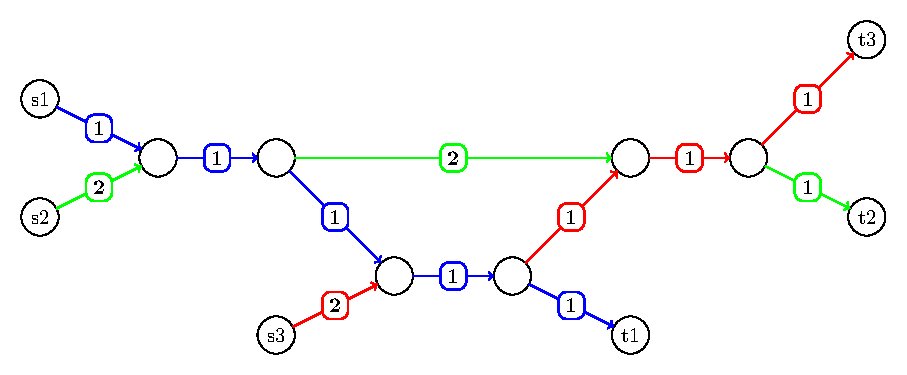
\includegraphics[scale=0.7]{Fig5.pdf}
      \end{center}
       \caption{A routage graph with $(0,\dots,0)$ as a $(2,1)$-periodic affectation}
      \end{figure}




   \subsection{Problems}

    We want to ensure that there is an affectation which allows to send periodic messages from elements in $S$ to elements in $L$.
    The problem we need to solve is thus the following:
    

      \noindent {\bf  Periodic Routes Assignment (PRA)} 

      \noindent {\bf Input:} a routage graph $\cal R$, an integer $\tau$ and an integer $P$.

      \noindent {\bf Question:} does there exist a $(P,\tau)$-periodic affectation of $\cal R$ ?

      We will prove in Sec.~\ref{sec:complexity} that the problem PRA is $\NP$-complete, even in restricted settings.
      Even approximating the smallest value of $P$ for which there is a $P$-periodic assignment is hard.
      Another strange property is that given a routage graph, we may have a $(P,\tau)$-periodic affectation but no
      $(P',\tau)$-periodic affectation with $P' > P$, the property is thus not monotone with regards to $P$.

	\begin{lemma} 
	 For any $P$, there is a routage graphe such that there is $(2,1)$-periodic affectation but no $(P,1)$-periodic affectation.
	\end{lemma}
\begin{proof}
      Consider the routage graph ${\cal R}$ given in the previous subsection. 
      We change the delays so that for $v$ the first vertex which belong to $r_i$ and $r_j$,
      we have $\lambda(v,r_i) - \lambda(v,r_j)= P$, where $P$ is an odd number smaller than $c$ the number of routes in ${\cal R}$.
      If we consider a period of $2$, for all $i \neq j$, $\lambda(v,r_i) - \lambda(v,r_j) = 1 $ modulo $2$. Therefore $(0,\dots,0)$ is a $(2,1)$-periodic affectation of ${\cal R}$.
      On the other hand, if we want to find a $(P,1)$-periodic affectation, then $\lambda(v,r_i) - \lambda(v,r_j) = 0 $ modulo $P$.
      Thus we must find $m_i \in \{0,\dots,P-1\}$ such that for all $i \neq j \in \{1,\dots,c\}^2$, $m_i \neq m_j$, which is impossible since $P < c$. 
      
\end{proof}
      
% 
%       \begin{figure}[H]
%       \label{could-ran}
%       \begin{center}
%       % \begin{tabular}{cc}
%       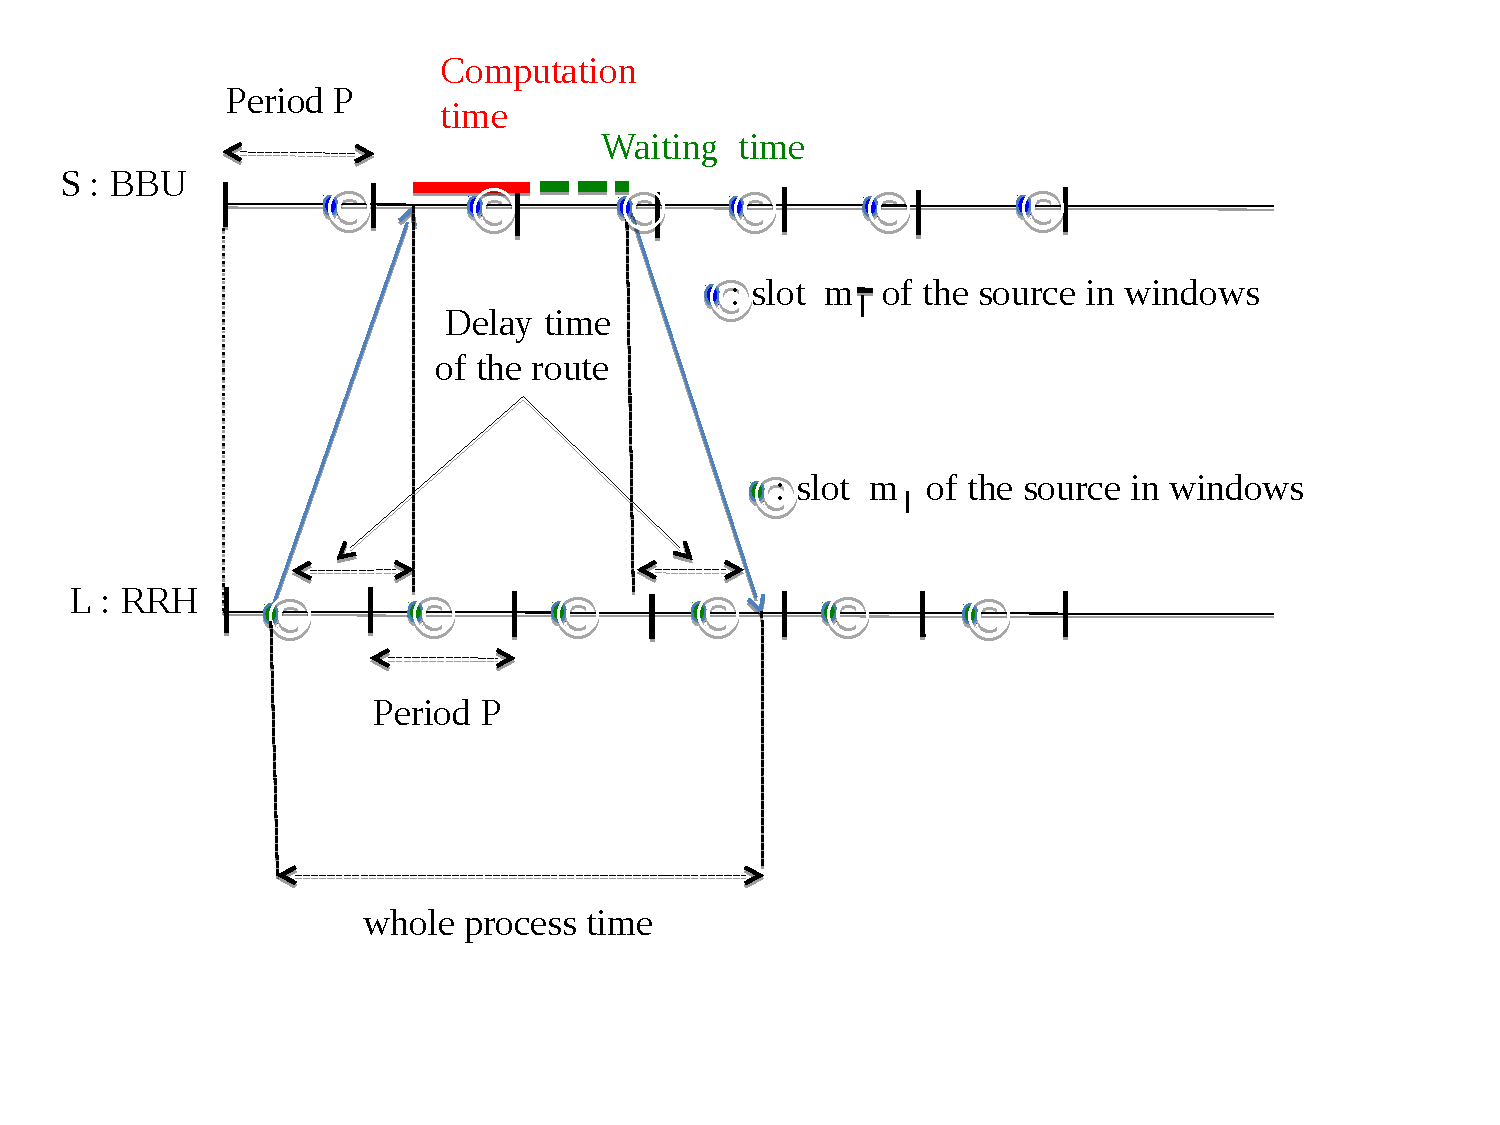
\includegraphics[scale=0.5]{Total-latence.pdf}
%       \caption{Complete process for a leaf in $L$.}
%       \end{center}
%       \end{figure}
%       %\end{tabular}\newline

      
      In the context of cloud-RAN applications, we consider here the digraph $G=(V,A)$ modeling the target network 
      and two disjoint subsets of vertices $S$ and $L$, where $S$ is the set of BBU and $L$ is the set of RRH. 
      We denote by $n$ the size of $S$ and $L$. We are given a period $P$, a routing function ${\cal R}$ and a bijection $\rho:L\rightarrow S$ which assigns a BBU to each RRH. Let ${\cal C}_{\rho} = \{(l,\rho(l))\}_{l \in L} \cup \{(s,\rho^{-1}(s))\}_{s \in S}$. Let consider a $P$-periodic affectation of ${\cal C}_{\rho}$ which associates $m_l$ to 
      $(l,\rho(l))$ and $m_{\rho(l)}$ to $(\rho(l),l)$.  
      
      This affectation represents the following process: first a message is sent in $l$, through the route $r_l$, at time $m_l$.
      
      \begin{center}
      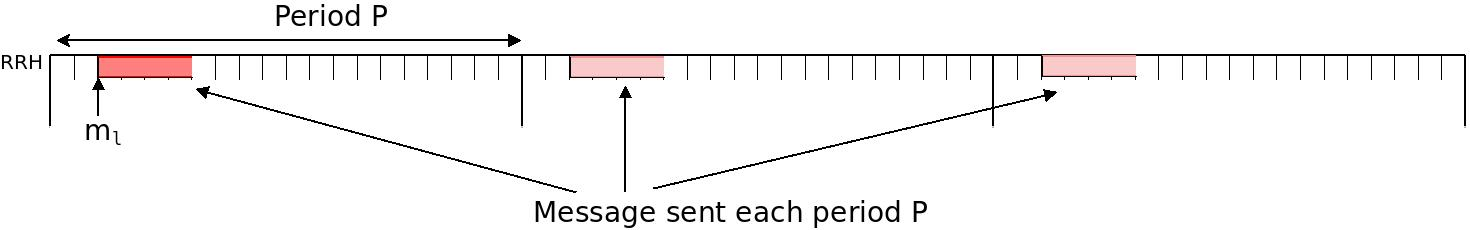
\includegraphics[scale=0.2]{rrh.jpeg}
      \end{center}
      
      This message is received by $\rho(l)$ at time $t(\rho(l),r_l)$. It is then sent back to $l$ in the same period at time $m_{\rho(l)}$ if $m_{\rho(l)} > t(\rho(l),r_l)$, otherwise at time $m_{\rho(l)}$ in the next period. The time between the arrival of the message and the time it is sent back is called the \textbf{waiting time} and is defined by $w_l = m_{\rho(l)} - t(\rho(l),r_l)$ if $m_{\rho(l)} > t(\rho(l),r_l)$ and $w_l = m_{\rho(l)} + P - t(\rho(l),r_l)$ otherwise.
      
       \begin{center}
      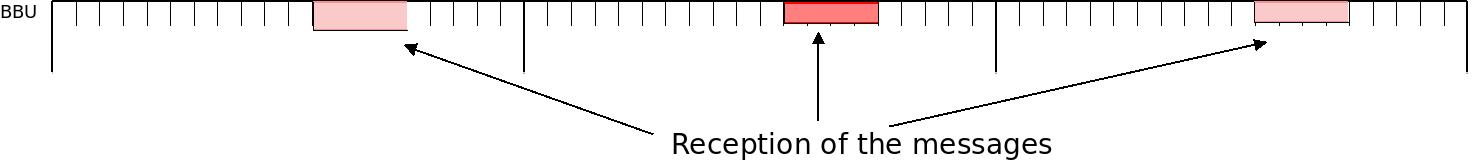
\includegraphics[scale=0.2]{BBU1.jpeg}
      
      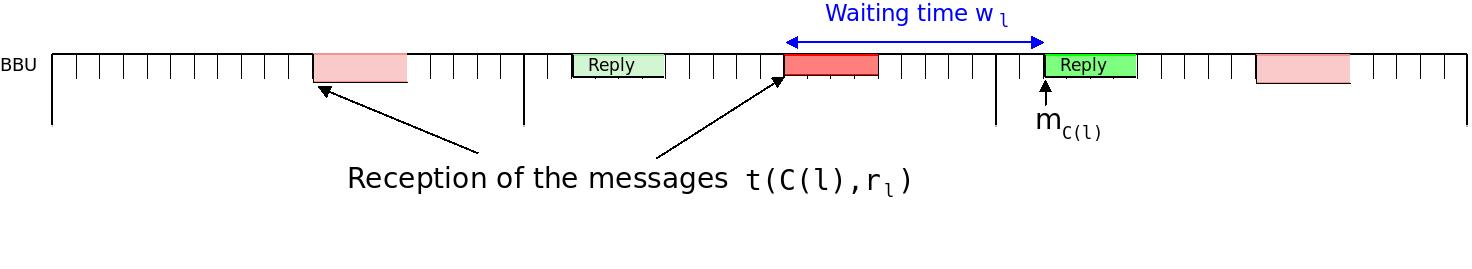
\includegraphics[scale=0.2]{BBU2.jpeg}
      \end{center}
     
      
      When a BBU receives a message, it must compute the answer before sending it back to the RRH. This time can be encoded
      in the last arc leading to the BBU and thus we need not to consider it explicitely in our model.
    
      Thus, the whole proccess time for a vertex $l$ is equal to
      $$
      PT(l)=\lambda(r_l)+ w_l+\lambda(r_{\rho(l)}).
      $$
      
    The {\bf maximum process time} of the $P$-periodic affectation ${\cal M} $ is defined by $MT({\cal M})=\max\limits_{l \in L} PT(l)$. The problem we want to solve is the following. 

      \noindent {\bf Problem Periodic Assignment for Low Latency(PALL)} 

      \noindent {\bf Input:}  a digraph $G$, a matching $\rho$ from $L$ to $S$ two disjoint set of vertices of $G$, a routing function $\cal R$, a period $P$, an integer $T_{max}$.

      \noindent {\bf Question:} does there exist a $P$-periodic affectation ${\cal M}$ of ${\cal C}_{\rho}$ in $(G,{\cal R})$ such that $MT({\cal M}) \leq T_{max}$?

      %The related optimisation problem we will focus on  consists in minimizing  $MT({\cal M})$. Note that in the context of cloud-RAN networks, we consider $P=1ms$, $\theta=2.6ms$ and $T_{max}$ must be less or equal to $3ms$.
      %cette remarque doit être dans la partie expérimentale



  
\section{Solving PRA}
  \label{sec:complexity}
  \subsection{NP-Hardness}

 In this section we assume that the size of a message $\tau$ is equal to one, which implies hardness of PRA and PALL for all $\tau$. 
Consider an instance of Problem PRA, i.e., a digraph $G=(V,A)$, an assignment $\cal C$, a routing function $\cal R$ and a period $P$. 
The {\bf conflict depth} of a route is the number of other routes which share an edge with it. 
The conflict depth of an assignment $\cal C$ is the maximum of the conflict depth of the routes in ${\cal R}_{\cal C}$.
The {\bf load} of an assignment is the maximal number of routes sharing the same arc.
It is clear that a $P$-periodic affectation must satisfy that $P$ is larger or equal to the load.

We give two alternate proofs that PRA is $\NP$-complete.
The first one works for conflict depth $2$ and is minimal in this regards since we later prove that for conflict depth one,
it is easy to solve PRA. The second one reduces the problem to graph coloring and implies inapproximability when one tries to minimize the parameter $P$. \\
 

 

 \begin{proposition}
Problem PRA is $\NP$-complete, when the routing is of conflict depth two.
\end{proposition}
 \begin{proof}
 The problem $PRA$ is in $\NP$ since given an offfset for each route in an affectation, it is easy to check in linear time in the number of edges whether there are collisions.
 
  Let $H=(V,E)$ be a graph and let $d$ be its maximal degree. We consider the problem to determine whether $H$ is edge-colorable
  with $d$ or $d+1$ colors. The edge coloring problem is $\NP$-hard~\cite{holyer1981np} and we reduce it to PRA to prove its $\NP$-hardness. We define from $H$ an instance of PRA as follows. The graph $G$ has for vertices $V'= \{ v_1, v_2 \mid v \in V  \} \cup \{ l_{u,v}, s_{u,v} \mid (u,v) \in E \}$ that is two vertices for each vertex and for each edge of $H$. 
  Let $A$ bet the set of arcs of $G$, defined by 
  $$A = \{(v_1,v_2) \mid v\in V\} \cup \{(u_2,v_1)\mid u \neq v \in V^2\} \cup \{(l_{u,v},u_1),(v_2,s_{u,v}) \mid (u,v) \in E \}. $$
  All these arcs are of weigth $0$. 
  For each edge $(u,v) \in E$, the is a route $r_{u,v} = s_{u,v},u_1,u_2,v_1,v_2,l_{u,v}$ in ${\cal R}$.  
  The affectation ${\cal C}$ is the set of pair of vertices $(s_{u,v}, l_{u,v})$.
    
  Observe that the existence of a $d$-coloring of $H$ is equivalent to the existence of a $d$-periodic affectation
  for $(G,{\cal R},{\cal C})$. Indeed, a $d$-coloring of $H$ can be seen as a labeling of its edges by the integers
  in $\{0,\dots,d-1\}$ and we have a correspondance between a $d$-coloring of $H$ and offests for the routes of $(G,{\cal R},{\cal C})$.
  By contruction, the constraint of having no collision between the routes is equivalent to the fact that no two adjacent edges have
  the same color. Therefore we have reduced edge coloring to PRA which concludes the proof. 
 \end{proof}
 \todo{Faire un dessin d'illustration ?}
 
 Remark that we have used zero weigth in the proof. If the weigths must be strictly positive, which makes more sense in our model since
 we model the latency of physical links, it is easy to adapt the proof. We just have to set them so that in any route the delay at $u_1$ is equal to $d$ and thus equal to $0$ modulo $d$. We now lift this hardness result to the problem PALL.

\begin{corollary}
Problem PALL is $\NP$-complete for routing of conflict depth two.
\end{corollary}
\begin{proof}
 We consider $(G,{\cal R},{\cal C},P)$ an instance of $PRA$ such that no element appears both in the first and second position in a pair of ${\cal C}$. Remark that this condition is satisfied in the previous proof, which makes the problem $PRA$ restricted to these instances $\NP$-complete. 
 Let us define $T_{max} = 2 \times \max_{r \in {\cal R}} \lambda(r) + P$. We define $\rho$ as the function which maps 
 $u$ to $v$ when $(u,v) \in {\cal C}$. The instance $(G,{\cal R},\rho,P,T_{max})$ is in PALL if and only if $(G,{\cal R},{\cal C},P)$
 is in $PRA$. Indeed the waiting time of each route is by definition less than $P$ and thus the maximal process time less than $T_{max}$. Therefore the fact that $(G,{\cal R},\rho,P,T_{max})$ is in PALL is equivalent to the existence of a $P$-periodic assignment of ${\cal C}_{\rho}$ which is equal to ${\cal C}$.
\end{proof}
% 
% 
% As another corollary of the previous proposition,  given $G$, $\cal R$, $P$ and two disjoint subsets $S$ and $L$ in $G$, the problem of  knowing if there is a matching $\rho$  from $L$ in $S$ such that the answer to problem PRA for instance $G,{\cal C_{\rho}},{\cal R}, P$ is  $\NP$-hard since checking a potential feasible solution for this problem implies to solve PRA.\\

Let MIN-PRA be the problem, given a graph, a routing and an affectation, to find the minimal period $P$ such that there is a $P$-periodic affectation. 

\begin{theorem}
 The problem MIN-PRA cannot be approximated in polynomial time within a factor $n^{1-o(1)}$, with $n$ the number of routes, unless $\P = \NP$ even when the load is two.
\end{theorem}

\begin{proof}
 We reduce graph coloring to PRA. Let $H$ be a graph instance of the $k$-coloring problem. 
 We define $G$ in the following way: for each vertex $v$ in $H$, there is a route $r_v$ in $G$.
 Two routes $r_v$ and $r_u$ share an arc if and only if $(u,v)$ is an edge in $H$; this arc is the only one shared by these two routes.   
 All arcs are of delay $0$. 
 
 Observe that the existence of a $k$-coloring of $H$ is equivalent to the existence of a $k$-periodic affectation in $G$, 
 by converting an offset of a route into a color of a vertex and reciprocally. Therefore if we can approximate the minimum value of $P$ within a factor $f$,
 we could approximate the minimal number of colors needed to color a graph within a factor $f$, by doing the previous reduction for all possible $k$. The proof follows from the hardness of approximability of finding a minimal coloring~\cite{zuckerman2006linear}.
\end{proof}


In particular, this reduction shows that even with small maximal load, the 
minimal period can be large.

    \scalebox{0.5}{

    \begin{tikzpicture}

    \tikzset{
      LabelStyle/.style = { rectangle, rounded corners, draw,
			  font = \bfseries },
      EdgeStyle/.append style = {->} }
      \SetGraphUnit{5}
      \Vertex[x=4,y=2]{s3}
      \Vertex[x=0,y=4]{s2}
      \Vertex[x=0,y=6]{s1}
      
      \Vertex[x=12,y=3]{l3}
      \Vertex[x=14,y=4]{l2}
      \Vertex[x=10,y=2]{l1}
      \tikzstyle{VertexStyle}=[shape = circle, draw, minimum size = 20pt]
	\tikzset{
      VertexStyle/.append style = {blue} }
	\Vertex[x=-8,y=3]{1}
	      \tikzset{
      VertexStyle/.append style = {green} }
	  \Vertex[x=-7,y=5]{2}

	    \tikzset{
      VertexStyle/.append style = {red} }
	  \Vertex[x=-6,y=4]{3}
		\tikzset{
      VertexStyle/.append style = {black} }
      
      
      \SetVertexNoLabel
      \Vertex[x=2,y=5]{A}
      \Vertex[x=4,y=5]{B}
      \Vertex[x=10,y=5]{C}
      \Vertex[x=12,y=5]{D}
      \Vertex[x=6,y=3]{E}
      \Vertex[x=8,y=3]{F}
      \tikzset{
      EdgeStyle/.append style = {green} }
      \Edge[label = 3](s2)(A)
      \Edge(A)(B)
      \Edge(B)(C)
      \Edge(C)(D)
      \Edge(D)(l2)

      
      \tikzset{
      EdgeStyle/.append style = {red} }
      \Edge[label = 1](s3)(E)
      \Edge(E)(F)
      \Edge(F)(l3) 
	\tikzset{
      EdgeStyle/.append style = {blue} }
      \Edge[label = 1](s1)(A)
      \Edge[label = 1](A)(B)
      \Edge[label = 1](B)(E)
      \Edge(E)(F)
      \Edge(F)(l1)
      
	\tikzset{
      EdgeStyle/.append style = {black,-} }

      \Edge(1)(2)
      \Edge(1)(3)
    \node (1) at (-3,4){\Huge $\rightarrow$};
    
    \node (2) at (-7,-2){\Huge G};
    \node (3) at (10,-2){\Huge H};
    \end{tikzpicture}


    }
    
    
  \subsection{MIN-PRA}
    Exemple de cas polynomiaux
    
\section{The Star Topolgy}
  
  In this section, we consider a particular case of the model, in which for each $(u,v)$ , the route is the same in both directions. This means that ${\cal R}(u,v)$ uses the same arcs as ${\cal R}(v,u)$ in the opposite orientation.
  \subsection{Intro}
    PALL NP-Hard car PRA NP-Hard\\
    Résultats valables sur Topologie 1 avec nos paramètres
    \todo{J'ai viré star affectation, car je pense qu'il n'y a rien à dire là dessus.}
    
  \subsection{No waiting times}
    \subsubsection{Shortest-longest}
      \paragraph{Algo}
      \paragraph{Period}
    \subsubsection{Greedy Algorithm with higher bound}
   
	\begin{algorithm}[H]
	\caption{Greedy with Higher bound Period(GHP)}
	\begin{algorithmic}
	\REQUIRE ${\cal R}_{\cal C}$, period $P$
	\ENSURE A P-periodic affectation in p $\leq P$, or FAILURE
	\STATE $P1[P]$ slots of size $\tau$ in first way period.
	\STATE $P2[P]$ slots  of size $\tau$ in back way period.
	\FORALL{route i in ${\cal R}_{\cal C}$ }

	\FORALL{slot j in P1}

	\IF{$P1[j]$ is free AND $P2[j+\lambda(r_i)]$ is free}

	
	\STATE $o_i \leftarrow j$
	\ENDIF


	\IF{No intervals are found for i}
	\STATE return FAILURE
	\ENDIF
	\ENDFOR

	\ENDFOR

	\end{algorithmic}
	\end{algorithm}
      \paragraph{Period}
	This algorithm gives us a solution without waiting times in a maximum period $3.\tau.c$, if we have $c$ routes.\\
	Suppose that we have a period of $3.\tau.c$ slots, divided in $\tau$ macro-slots. Let us call {\em forward period} the period in the central node when the messages goes to RRH to BBU, and {\em backward period} the period when the messages comes back in the other way. Put a message in the first slot of size $\tau$ in the forward period, such that the corresponding area in the backward period is free.This message takes at most 2 slots of time $\tau$ in the backward period.\\
	\todo{Dessin qui illustre ça}\\
	When $k < c$ messages are put in the forward period, and we want to add another message, there is $3.c - k$ free slots of size $\tau$ in the forward period. Those $3.c - k$ gives us $3.c - k$ possible slots in the backward periods.\\
	The $k$ messages uses at most $2k$ slots of size $\tau$ used in the backward period. Since $k<c$,  $2k < 3.c - k$, thus using the pigeonhole principle, there is at least one free slot in the backward period for the new message.
	
    \subsubsection{Exhaustive generation}
      Décrire l'algo, expliquer les coupes
    \subsubsection{Results}
      Resultats des simulations : Shortest-longest optimal pour ces parametres.
      
   \subsection{Allowing waiting times}
     \subsubsection{Intro}
	Importance des waiting times quand la période est donnée (Résultats D'éxepriences et preuve avec l'exemple)
     \subsubsection{LSG}
	\paragraph{Algorithm}
	\paragraph{Analysis}
	  Parler de LSO et expliquer pourquoi LSG mieux avec nos params
     \subsubsection{Results}
	 \paragraph{Random}
	 \paragraph{Distributions}
   
\section{Conclusion}

\bibliographystyle{plain}
\bibliography{Sources.bib}


\end{document}
